% Introduction chapter.
%
% Developed for my Master Thesis at Maastricht University.
% Based on Eugenio Senes's template at the University of Torino.
%
% By Joeri Hermans (joeri@joerihermans.com)
%
% Released under an MIT license. Share, modify and enjoy, but quote the author!

\chapter{Introduction}
\label{chapter:introduction}

In this chapter we introduce Distributed Deep Learning and the problems surrounding it. A more detailed description of the subject of study is given in Chapter~\ref{chapter:distributed_deep_learning}. Furthermore, we make the reader more comfortable with the notation and abbreviations used throughout this thesis. Finally, we formally define the problem statement in Section~\ref{sec:problem_statement}, and give an outline of this thesis in Section~\ref{sec:thesis_outline}.

\section[Distributed Deep Learning]{Distributed Deep Learning, an introduction}
\label{sec:intro_distributed_deep_learning}

Unsupervised feature learning and deep learning has shown that being able to train large models can drastically improve model performance. However, consider the problem of training a deep network with millions, or even billions of parameters. How do we achieve this without waiting for days, or even multiple weeks? Dean et al.~propose a different training paradigm which allows us to train and serve a model on multiple physical machines~\cite{dean2012large}. The authors propose two novel methodologies to accomplish this. Namely, \emph{model parallelism}, introduced in Section~\ref{sec:intro_model_parallelism}, and \emph{data parallelism}, introduced in Section~\ref{sec:intro_data_parallelism}.\\

In this thesis we study \emph{data parallelism}, since this methodology mainly focuses on the development of distributed optimization algorithms. Whereas, \emph{model parallelism} is mainly an engineering effort, because it still follows the traditional optimization scheme, i.e., sequential gradient updates in the case the applied optimizer utilizes a gradient based approach.

\subsection{Model Parallelism}
\label{sec:intro_model_parallelism}

In \emph{model parallelism}, a single model is distributed over multiple machines~\cite{dean2012large}. The performance benefits of distributing a deep network across multiple machines mainly depends on the structure of the model. Models with a large number of parameters typically benefit from access to more CPUs and memory, up to the point where communication costs, i.e., propagation of weight updates and synchronization mechanisms, dominate~\cite{dean2012large}.\\

Let us start with a simple example in order to illustrate this concept more clearly. Imagine having a perceptron, as depicted in Figure~\ref{fig:introduction_model_parallelism_perceptron}. In order to parallelize this efficiently, we can view a neural network as a dependency graph, where the goal is to minimize the number of synchronization mechanisms, assuming we have unlimited resources. Furthermore, a synchronization mechanism is only required when a node has more than 1 \emph{variable} dependencies. A variable dependency is a dependency which can change in time. For example, a bias would be a \emph{static} dependency, because the value of a bias remains constant over time. In the case for the perceptron shown in Figure~\ref{fig:introduction_model_parallelism_perceptron}, the parallelization is quite straightforward. The only synchronization mechanism which should be implemented resides in output neuron since $y \triangleq \sigma(\sum_i w_ix_i$) where $\sigma$ is the activation function of the output neuron.

\begin{figure}[H]
  \centering
  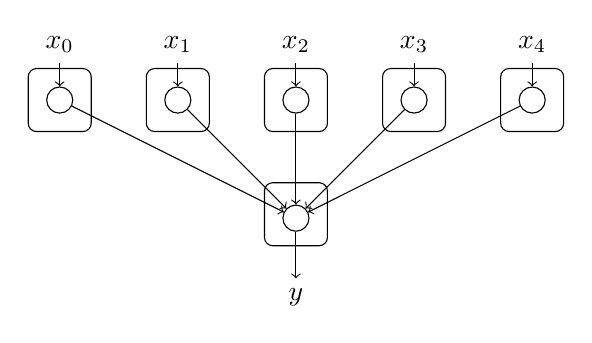
\begin{tikzpicture}

    % Draw inputs.
    \node (i_0) at (-3, 0.7) {$x_0$};
    \node (i_1) at (-1.5, 0.7) {$x_1$};
    \node (i_2) at (0, 0.7) {$x_2$};
    \node (i_3) at (1.5, 0.7) {$x_3$};
    \node (i_4) at (3, 0.7) {$x_4$};


    % Draw the input neurons.
    \node[circle, minimum size=0.2cm, thin, draw=black] (1) at (-3,0) {};
    \node[circle, minimum size=0.2cm, thin, draw=black] (2) at (-1.5,0) {};
    \node[circle, minimum size=0.2cm, thin, draw=black] (3) at (0,0) {};
    \node[circle, minimum size=0.2cm, thin, draw=black] (4) at (1.5,0) {};
    \node[circle, minimum size=0.2cm, thin, draw=black] (5) at (3,0) {};

    % Draw the output neuron.
    \node[circle, minimum size=0.2cm, thin, draw=black] (6) at (0, -1.5) {};

    % Draw output.
    \node (y) at (0, -2.5) {$y$};

    % Draw the lines.
    % X -> Input.
    \draw[->] (i_0) -- (1);
    \draw[->] (i_1) -- (2);
    \draw[->] (i_2) -- (3);
    \draw[->] (i_3) -- (4);
    \draw[->] (i_4) -- (5);
    % Input -> Output.
    \draw[->] (1) -- (6);
    \draw[->] (2) -- (6);
    \draw[->] (3) -- (6);
    \draw[->] (4) -- (6);
    \draw[->] (5) -- (6);
    % Output.
    \draw[->] (6) -- (y);

    % Draw the nodes.
    \draw[rounded corners=3pt] (-3.4,0.4) rectangle ++(0.8,-0.8);
    \draw[rounded corners=3pt] (-1.9,0.4) rectangle ++(0.8,-0.8);
    \draw[rounded corners=3pt] (-0.4,0.4) rectangle ++(0.8,-0.8);
    \draw[rounded corners=3pt] (1.1,0.4) rectangle ++(0.8,-0.8);
    \draw[rounded corners=3pt] (2.6,0.4) rectangle ++(0.8,-0.8);
    \draw[rounded corners=3pt] (-0.4,-1.05) rectangle ++(0.8,-0.8);
  \end{tikzpicture}
  \caption{A perceptron partitioned using the \emph{model parallelism} paradigm. In this approach every input node is responsible for accepting the input $x_i$ from some source, and multiplying the input with the associated weight $w_i$. After the multiplication, the result is sent to the node which is responsible for computing $y$. Of course, this node requires a synchronization mechanism to ensure that the result is consistent. The synchronization mechanism does this by waiting for the results $y$ depends on.}
  \label{fig:introduction_model_parallelism_perceptron}
\end{figure}

\subsection{Data Parallelism}
\label{sec:intro_data_parallelism}

In this thesis, we focus our efforts on data parallelism. Data parallelism is an inherently different methodology of optimizing parameters. The general idea is to reduce the training time by having $n$ different workers optimizing a model by processing $n$ different shards (partitions) of the dataset in parallel~\cite{dean2012large}. In this setting we distribute $n$ model replicas over $n$ processing nodes, i.e., every node (or process) holds one model replica. Then, the workers train their local replica using the assigned data shard. However, it is possible to coordinate the workers in such a way that, together, they will optimize a single objective. There are several approaches to achieve this, and these will be discussed in greater detail in Chapter~\ref{chapter:distributed_deep_learning}.\\

Nevertheless, a popular approach to optimize this objective, is to employ a centralized \emph{parameter server}~\cite{dean2012large, zhang2015deep, recht2011hogwild}. A parameter server is responsible for the aggregation of model updates, and parameter requests coming from different workers. The distributed learning process starts by partitioning a dataset into $n$ \emph{shards}. Every individual shard will be assigned to a particular worker. Next, a worker will sample mini-batches from its shard in order to train the local model replica. After every mini-batch (or multiple mini-batches), the workers will communicate a variable with the parameter server. This variable is in most implementations the gradient $\nabla f_i(x)$. Finally, the parameter server will integrate this variable by applying a specific \textsc{update} procedure which knows how to handle this variable. This process repeats itself untill all workers have sampled all mini-batches from their shard. The above high level description is summarized in Figure~\ref{fig:introduction_data_parallelism_schematic}.\\



\begin{figure}[H]
  \centering
  % Define database shape.
  \def\database at (#1,#2){
    \draw (#1,#2) ellipse (0.5 and 0.15);
    \draw (#1 - 0.5, #2) -- (#1 - 0.5, #2 - 1);
    \draw (#1 + 0.5, #2) -- (#1 + 0.5, #2 - 1);
    \draw (#1 - 0.5, #2 - 1/3) arc (180:360:0.5 and 0.15);
    \draw (#1 - 0.5, #2 - 2/3) arc (180:360:0.5 and 0.15);
    \draw (#1 - 0.5, #2 - 1) arc (180:360:0.5 and 0.15);
  }
  % Define datashard shape.
  \def\datashard at (#1,#2){
    \draw (#1,#2) ellipse (0.5 and 0.15);
    \draw (#1 - 0.5, #2) -- (#1 - 0.5, #2 - 1/3);
    \draw (#1 + 0.5, #2) -- (#1 + 0.5, #2 - 1/3);
    \draw (#1 - 0.5, #2 - 1/3) arc (180:360:0.5 and 0.15);
  }
  % Define the neural network shape.
  \def\neuralnet at (#1,#2){
    % Draw node bounding box.
    \draw[rounded corners=3pt] (#1 - 0.7,#2 + 0.5) rectangle ++(1.4,-0.95);
    % Draw fully connected lines.
    \draw[gray] (#1 + 0.25,#2) -- (#1 - 0.375, #2 + 0.25);
    \draw[gray] (#1 + 0.25,#2) -- (#1 - 0.125, #2 + 0.25);
    \draw[gray] (#1 + 0.25,#2) -- (#1 + 0.125, #2 + 0.25);
    \draw[gray] (#1 + 0.25,#2) -- (#1 + 0.375, #2 + 0.25);
    \draw[gray] (#1 + 0.5,#2) -- (#1 - 0.375, #2 + 0.25);
    \draw[gray] (#1 + 0.5,#2) -- (#1 - 0.125, #2 + 0.25);
    \draw[gray] (#1 + 0.5,#2) -- (#1 + 0.125, #2 + 0.25);
    \draw[gray] (#1 + 0.5,#2) -- (#1 + 0.375, #2 + 0.25);
    \draw[gray] (#1,#2) -- (#1 - 0.375, #2 + 0.25);
    \draw[gray] (#1,#2) -- (#1 - 0.125, #2 + 0.25);
    \draw[gray] (#1,#2) -- (#1 + 0.125, #2 + 0.25);
    \draw[gray] (#1,#2) -- (#1 + 0.375, #2 + 0.25);
    \draw[gray] (#1 - 0.25,#2) -- (#1 - 0.375, #2 + 0.25);
    \draw[gray] (#1 - 0.25,#2) -- (#1 - 0.125, #2 + 0.25);
    \draw[gray] (#1 - 0.25,#2) -- (#1 + 0.125, #2 + 0.25);
    \draw[gray] (#1 - 0.25,#2) -- (#1 + 0.375, #2 + 0.25);
    \draw[gray] (#1 - 0.5,#2) -- (#1 - 0.375, #2 + 0.25);
    \draw[gray] (#1 - 0.5,#2) -- (#1 - 0.125, #2 + 0.25);
    \draw[gray] (#1 - 0.5,#2) -- (#1 + 0.125, #2 + 0.25);
    \draw[gray] (#1 - 0.5,#2) -- (#1 + 0.375, #2 + 0.25);
    \draw[gray] (#1 + 0.25,#2) -- (#1 + 0.125, #2 - 0.25);
    \draw[gray] (#1 + 0.25,#2) -- (#1 - 0.125, #2 - 0.25);
    \draw[gray] (#1 + 0.5,#2) -- (#1 + 0.125, #2 - 0.25);
    \draw[gray] (#1 + 0.5,#2) -- (#1 - 0.125, #2 - 0.25);
    \draw[gray] (#1,#2) -- (#1 + 0.125, #2 - 0.25);
    \draw[gray] (#1,#2) -- (#1 - 0.125, #2 - 0.25);
    \draw[gray] (#1 - 0.25,#2) -- (#1 + 0.125, #2 - 0.25);
    \draw[gray] (#1 - 0.25,#2) -- (#1 - 0.125, #2 - 0.25);
    \draw[gray] (#1 - 0.5,#2) -- (#1 + 0.125, #2 - 0.25);
    \draw[gray] (#1 - 0.5,#2) -- (#1 - 0.125, #2 - 0.25);
    % Define input layer.
    \draw[fill=white] (#1 - 0.375,#2 + 0.25) circle (1pt);
    \draw[fill=white] (#1 - 0.125,#2 + 0.25) circle (1pt);
    \draw[fill=white] (#1 + 0.125,#2 + 0.25) circle (1pt);
    \draw[fill=white] (#1 + 0.375,#2 + 0.25) circle (1pt);
    % Define hidden layer.
    \draw[fill=white] (#1 - 0.5,#2) circle (1pt);
    \draw[fill=white] (#1 - 0.25,#2) circle (1pt);
    \draw[fill=white] (#1,#2) circle (1pt);
    \draw[fill=white] (#1 + 0.25,#2) circle (1pt);
    \draw[fill=white] (#1 + 0.5,#2) circle (1pt);
    % Define output layer.
    \draw[fill=white] (#1 - 0.125,#2 - 0.25) circle (1pt);
    \draw[fill=white] (#1 + 0.125,#2 - 0.25) circle (1pt);
  }
  \def\neuralnetclean at (#1,#2){
    \draw[gray] (#1 + 0.25,#2) -- (#1 - 0.375, #2 + 0.25);
    \draw[gray] (#1 + 0.25,#2) -- (#1 - 0.125, #2 + 0.25);
    \draw[gray] (#1 + 0.25,#2) -- (#1 + 0.125, #2 + 0.25);
    \draw[gray] (#1 + 0.25,#2) -- (#1 + 0.375, #2 + 0.25);
    \draw[gray] (#1 + 0.5,#2) -- (#1 - 0.375, #2 + 0.25);
    \draw[gray] (#1 + 0.5,#2) -- (#1 - 0.125, #2 + 0.25);
    \draw[gray] (#1 + 0.5,#2) -- (#1 + 0.125, #2 + 0.25);
    \draw[gray] (#1 + 0.5,#2) -- (#1 + 0.375, #2 + 0.25);
    \draw[gray] (#1,#2) -- (#1 - 0.375, #2 + 0.25);
    \draw[gray] (#1,#2) -- (#1 - 0.125, #2 + 0.25);
    \draw[gray] (#1,#2) -- (#1 + 0.125, #2 + 0.25);
    \draw[gray] (#1,#2) -- (#1 + 0.375, #2 + 0.25);
    \draw[gray] (#1 - 0.25,#2) -- (#1 - 0.375, #2 + 0.25);
    \draw[gray] (#1 - 0.25,#2) -- (#1 - 0.125, #2 + 0.25);
    \draw[gray] (#1 - 0.25,#2) -- (#1 + 0.125, #2 + 0.25);
    \draw[gray] (#1 - 0.25,#2) -- (#1 + 0.375, #2 + 0.25);
    \draw[gray] (#1 - 0.5,#2) -- (#1 - 0.375, #2 + 0.25);
    \draw[gray] (#1 - 0.5,#2) -- (#1 - 0.125, #2 + 0.25);
    \draw[gray] (#1 - 0.5,#2) -- (#1 + 0.125, #2 + 0.25);
    \draw[gray] (#1 - 0.5,#2) -- (#1 + 0.375, #2 + 0.25);
    \draw[gray] (#1 + 0.25,#2) -- (#1 + 0.125, #2 - 0.25);
    \draw[gray] (#1 + 0.25,#2) -- (#1 - 0.125, #2 - 0.25);
    \draw[gray] (#1 + 0.5,#2) -- (#1 + 0.125, #2 - 0.25);
    \draw[gray] (#1 + 0.5,#2) -- (#1 - 0.125, #2 - 0.25);
    \draw[gray] (#1,#2) -- (#1 + 0.125, #2 - 0.25);
    \draw[gray] (#1,#2) -- (#1 - 0.125, #2 - 0.25);
    \draw[gray] (#1 - 0.25,#2) -- (#1 + 0.125, #2 - 0.25);
    \draw[gray] (#1 - 0.25,#2) -- (#1 - 0.125, #2 - 0.25);
    \draw[gray] (#1 - 0.5,#2) -- (#1 + 0.125, #2 - 0.25);
    \draw[gray] (#1 - 0.5,#2) -- (#1 - 0.125, #2 - 0.25);
    % Define input layer.
    \draw[fill=white] (#1 - 0.375,#2 + 0.25) circle (1pt);
    \draw[fill=white] (#1 - 0.125,#2 + 0.25) circle (1pt);
    \draw[fill=white] (#1 + 0.125,#2 + 0.25) circle (1pt);
    \draw[fill=white] (#1 + 0.375,#2 + 0.25) circle (1pt);
    % Define hidden layer.
    \draw[fill=white] (#1 - 0.5,#2) circle (1pt);
    \draw[fill=white] (#1 - 0.25,#2) circle (1pt);
    \draw[fill=white] (#1,#2) circle (1pt);
    \draw[fill=white] (#1 + 0.25,#2) circle (1pt);
    \draw[fill=white] (#1 + 0.5,#2) circle (1pt);
    % Define output layer.
    \draw[fill=white] (#1 - 0.125,#2 - 0.25) circle (1pt);
    \draw[fill=white] (#1 + 0.125,#2 - 0.25) circle (1pt);
  }
  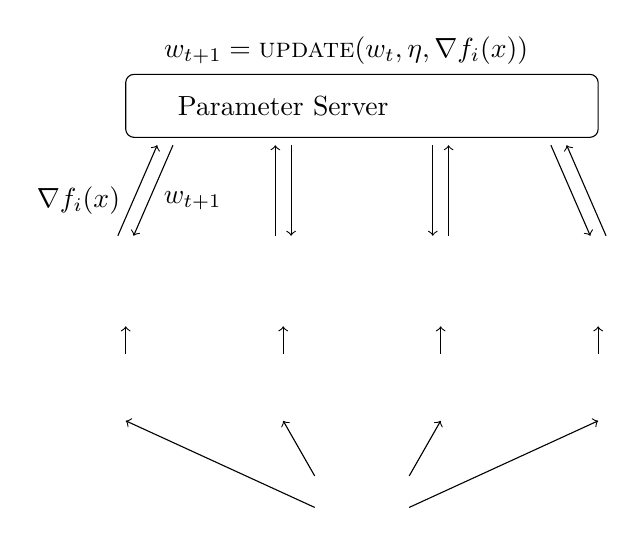
\begin{tikzpicture}
    \database at (0,0);
    \draw[->] (-0.6,-0.5) -- (-3, 0.6);
    \draw[->] (-0.6,-0.1) -- (-1, 0.6);
    \draw[->] (0.6,-0.1) -- (1, 0.6);
    \draw[->] (0.6,-0.5) -- (3, 0.6);
    \datashard at (-3,1.2)
    \datashard at (-1,1.2);
    \datashard at (1,1.2);
    \datashard at (3,1.2);
    \draw[->] (-3, 1.45) -- (-3, 1.8);
    \draw[->] (-1, 1.45) -- (-1, 1.8);
    \draw[->] (1, 1.45) -- (1, 1.8);
    \draw[->] (3, 1.45) -- (3, 1.8);
    \neuralnet at (3,2.35);
    \neuralnet at (1,2.35);
    \neuralnet at (-1,2.35);
    \neuralnet at (-3,2.35);
    % Draw the parameter server.
    \draw[rounded corners=3pt] (-3, 5) rectangle ++(6,-0.8);
    \node (pslabel) at (-1, 4.6) {Parameter Server};
    \node (psequation) at (-0.2, 5.3) {$w_{t+1} = \textsc{update}(w_t, \eta, \nabla f_i(x))$};
    % Draw the lines.
    \neuralnetclean at (1.8, 4.6);
    \draw[->] (-3.1, 2.95) -- (-2.6, 4.1);
    \draw[<-] (-2.9, 2.95) -- (-2.4, 4.1);
    \draw[->] (-1.1, 2.95) -- (-1.1, 4.1);
    \draw[<-] (-0.9, 2.95) -- (-0.9, 4.1);
    \draw[->] (1.1, 2.95) -- (1.1, 4.1);
    \draw[<-] (0.9, 2.95) -- (0.9, 4.1);
    \draw[->] (3.1, 2.95) -- (2.6, 4.1);
    \draw[<-] (2.9, 2.95) -- (2.4, 4.1);
    % Draw the labels.
    \node (commit) at (-2.15, 3.4) {$w_{t+1}$};
    \node (pull) at (-3.6, 3.4) {$\nabla f_i(x)$};
    % More labels.
  \end{tikzpicture}
  \caption{Schematic representation of a data parallel approach. In this methodology we spawn $n$ workers (not necessarily on different machines), and assign a data shard (partition) of the dataset to every worker. Using this data shard, a worker $i$ will iterate through all mini-batches to produce a gradient, $\nabla f_i(x)$, for every mini-batch $x$. Next, $\nabla f_i(x)$ is send to the parameter server, which will incorperate the gradient using an~\textsc{update} mechanism.}
  \label{fig:introduction_data_parallelism_schematic}
\end{figure}

\section{Problem Statement}
\label{sec:problem_statement}

\section{Thesis Outline}
\label{sec:thesis_outline}
